\documentclass[aspectratio=169]{beamer}
\usetheme{FLUKA}
\usepackage[utf8]{inputenc}
\usepackage[english]{babel}
\usepackage[T1]{fontenc}

%%% Feel free to remove these lines - they are needed for these slides only
\usepackage{lipsum}
\usepackage{pgfplots}
\pgfmathdeclarefunction{gauss}{2}{
  \pgfmathparse{1/(#2*sqrt(2*pi))*exp(-((x-#1)^2)/(2*#2^2))}%
}
\usetikzlibrary{calc,positioning}
%%%

\title{Your lecture title}

% This template can be used both for the school lectures and
% your FLUKA-related talks:
%
% If the school location is defined
\location{Lanzhou}{2024}
% then it is printed in the bottom-right corner
% along with the host logo in the upper-right corner.
%
% Otherwise, if location is set to empty values, i.e.
% \location{}{}
% then no host logo is displayed and
% the current date is printed in the bottom-right corner
% in this case, the date can be modified in the standard way:
% \date{February 22, 2024}

\author{Your Name} % not displayed in the lecture slides

\AtBeginSection[]{%
  \begin{frame}<beamer>{Outline}
    \tableofcontents[currentsection]
  \end{frame}
}

\begin{document}

\begin{frame}[plain]
\maketitle
\end{frame}

\begin{frame}{Outline}
\tableofcontents
\end{frame}

\section{Fonts}
\begin{frame}{\secname}
  \framesubtitle<1>{Titlepage: title}
  \framesubtitle<2>{Titlepage: location and date}
  \framesubtitle<3>{Normal text}
  \framesubtitle<4>{Text in footer}
  \framesubtitle<5>{Header: slide title}
  \framesubtitle<6>{Header: slide subtitle}
  \framesubtitle<7>{Block title}
  \framesubtitle<8>{Block text}
  \framesubtitle<9>{Itemize/enumerate body}
  \framesubtitle<10>{Itemize/enumerate subbody}
  \framesubtitle<11>{Itemize/enumerate subsubbody}
  \foreach \aaa [count=\i from 1] in {title, date, normal text, author in foot, frametitle, framesubtitle, block title, block text, itemize/enumerate body, itemize/enumerate subbody, itemize/enumerate subsubbody} {
    \only<\i>{
      \usebeamerfont{\aaa}
      \showfont
    }
  }
\end{frame}


\section{Colours}

\begin{frame}{\secname}
  \centering
  \begin{tikzpicture}
    \def \nColumns {6};
    \def \baseWidth {0.6cm};
    \def \baseHeight {0.37267081cm};

    \foreach \color [count=\i from 0] in {text, bar, header, alert, keyword} {
      \coordinate (center_\color)
      at ({2*mod(\i, \nColumns)}, {2*div(\i, \nColumns)});
      \coordinate (rectangle_bottom_\color)
      at ($(center_\color) - (\baseWidth, \baseHeight)$);
      \coordinate (rectangle_top_\color)
      at ($(center_\color) + (\baseWidth, \baseHeight)$);

      \draw[fill=beamer@\color color, black] (rectangle_bottom_\color) rectangle (rectangle_top_\color);
      \node[below=0.5cm of center_\color] {\color};
    }
  \end{tikzpicture}
\end{frame}

\begin{frame}{\secname}
  \begin{itemize}
    \item Normal text
    \item Text with an \alert{emphasised phrase}
    \item Text with a \keyword{keyword}, like a \keyword{USRBIN} estimator
  \end{itemize}
\end{frame}

 \section{Math}
 \begin{frame}{\secname}{Equation}
   \centering
   \Huge
   $$
   u(\rho,t) = J_0(k\rho) \cos(2\pi f t)
   $$
 \end{frame}

 \begin{frame}{\secname}{Matrix}
   \centering
   \Huge
   $$
   \mu = \left(
     \begin{array}{ccc}
       \mu_{1} & -jk & 0 \\
       jk & \mu_{1} & 0 \\
       0 & 0 & 1
     \end{array}
   \right)
   $$
 \end{frame}

 \section{Blocks}
 \begin{frame}{\secname}
   \only<1>{
     \framesubtitle{Block}
     \begin{block}{Block title}
       \lipsum[4]
     \end{block}
   }
   \only<2>{
     \framesubtitle{Exampleblock}
     \begin{exampleblock}{Block title}
       \lipsum[4]
     \end{exampleblock}
   }
   \only<3>{
     \framesubtitle{Alertblock}
     \begin{alertblock}{Block title}
       \lipsum[4]
     \end{alertblock}
   }
 \end{frame}

\section{Examples}
 \begin{frame}{\secname}
   \only<1>{
     \framesubtitle{Enumerate}
     \begin{enumerate}
     \item \lipsum[1][1] %\lipsum[2][1]
     \item \lipsum[1][2] \lipsum[2][2]
     \item \lipsum[1][3] \lipsum[2][3]
     \end{enumerate}
   }
   \only<2>{
     \framesubtitle{Itemize}
     \begin{itemize}
     \item \lipsum[1][1] %\lipsum[2][1]
     \item \lipsum[1][2] \lipsum[2][2]
     \item \lipsum[1][3] \lipsum[2][3]
     \end{itemize}
   }
   \only<3>{
     \framesubtitle{Table}
     \centering
     \begin{tabular}{ccc}
       \toprule
        $A$ & $B$ & $A\mathbin{\oplus}B$ \\
       \midrule
       0 & 0 & 0 \\
       0 & 1 & 1 \\
       1 & 0 & 1 \\
       1 & 1 & 0 \\
       \bottomrule
      \end{tabular}
   }
   \only<4>{
     \framesubtitle{TikZ picture}
     \centering
     \begin{tikzpicture}
       \begin{axis}[
           height=0.7\textheight,
           width=0.8\linewidth,
           xlabel = {x {[\si{\cm}]}},
           ylabel = {y {[\si{\cm}]}},
           title = {Title},
           view={0}{90},
           colormap/hot,
           colorbar sampled,
           colorbar style={
             title = {Palette title},
             ylabel = {Value {[arb. units]}},
             samples=8,
           },
         ]
	\addplot3[surf] {x*y};
	\end{axis}
     \end{tikzpicture}
   }
   \only<5>{
     \framesubtitle{External graphics}
     \begin{block}{Heavy ion incident onto ATIC spectrometer}
       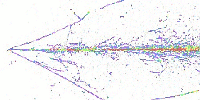
\includegraphics[width=0.49\linewidth]{figs/g1-soft.png} \hfill
       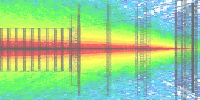
\includegraphics[width=0.49\linewidth]{figs/g5-soft.png}

       \hfill\copyr{http://www.fluka.org}{Toni Empl}
     \end{block}
   }
   \only<6>{
     \framesubtitle{\LaTeX\xspace template: {\tt \textbackslash keyword}, {\tt \textbackslash comment}, and {\tt \textbackslash alert}}
     The {\tt \textbackslash keyword} and {\tt \textbackslash comment} commands emphasise their arguments with different colours:
     \begin{itemize}
       \item {\tt \textbackslash keyword}\{USRBIN\} generates \keyword{USRBIN}
       \item {\tt \textbackslash comment}\{Some not-so-imporant info\} generates \comment{Some not-so-imporant info}
       \item Don't forget about the Beamer built-in command {\tt \textbackslash alert}\{Alerted text\} which generates \alert{Alerted text}
     \end{itemize}
   }
   \only<7>{
     \framesubtitle{\LaTeX\xspace template: {\tt \textbackslash card}}
     \begin{itemize}
     \item The {\tt\alert{\textbackslash card}} command provides an interface to typeset the FLUKA deck cards
     \item Syntax: {\tt \textbackslash card\{CARD\}\{WHAT1,WHAT2,\dots,WHAT6\}\{SDUM\}}
     \item An optional 4th argument adds the second line: \\
       {\tt \textbackslash card\{CARD\}\{WHAT1,WHAT2, \dots, WHAT6\}\{SDUM\}{[WHAT7,\dots,WHAT12]}}, i.e.
       \card{USRBIN}{-10.0, ELECTRON, -25.0, -7.0, 7.0, 12.1}{verythin}[-7.0,-7.0,12.0,35.0, ,1.0]
     \item The WHATs list is comma-separated and \alert{any {\tt WHAT}
       can be omitted} in the same way as in the free format input
     \item Use the \alert{tabular} environment if more than two deck lines are needed
     \end{itemize}
   }
   \only<8>{
     \framesubtitle{\LaTeX\xspace template: titlepage}
     It is possible to use this \LaTeX\xspace template for other FLUKA-related talks, without school information on the titlepage
     \begin{itemize}
       \item If the school location is defined, i.e., with {\tt
         \textbackslash location\{Lanzhou\}\{2024\}} then the
         corresponding info is printed in the bottom-right corner as
         it is done on the first slide
       \item Otherwise, if location is set to the empty values, i.e.,
         {\tt \textbackslash location\{\}\{\}} then no host info is
         displayed and the current date is printed in the bottom-right
         corner
         \begin{itemize}
         \item The date can be adjusted by the standard {\tt \textbackslash date} command
         \end{itemize}
       \item Contact KB if you have more suggestions about this template :)
     \end{itemize}

   }
 \end{frame}

 \section{Bibliography}
 \begin{frame}{\secname}
   \begin{thebibliography}{3}
     \beamertemplatearticlebibitems
   \bibitem{Tantau2010}
     Till Tantau, Joseph Wright, Vedran Mileti\'c
     \newblock The BEAMER class User Guide
     \newblock \href{http://bitbucket.org/rivanvx/beamer}{http://bitbucket.org/rivanvx/beamer}
     \newblock 2010

     \beamertemplatebookbibitems
   \bibitem{Book}
     Till Tantau
     \newblock{The TikZ and PGF Packages Manual}
     \newblock{\href{https://github.com/pgf-tikz/pgf}{https://github.com/pgf-tikz/pgf}}
     \newblock{2024}
   \end{thebibliography}
 \end{frame}

 \finalpage
\end{document}
